\chapter{Methode}

\section{Algoritmen}

In sectie \ref{bestaande-methoden} van deze scriptie zijn de voornaamste methoden waarmee datastreams gesynchroniseerd kunnen worden beknopt besproken. Hoewel de meeste algoritmen niet voldeden aan de vereisten bleken er twee toch zeer geschikt voor snelle en nauwkeurige synchronisatie van realtime streams. In dit gedeelte zullen deze methoden in detail worden behandeld. Ook wordt er onderzocht in welke mate het mogelijk is om deze algoritmes te combineren tot één systeem.

\subsection{Accoustic fingerprinting}
\label{accoustic-fingerprinting}

Bij het accoustic fingerprinting algoritme worden fingerprints geëxtraheerd uit audiofragmenten. Het zoek naar gelijkenissen gebeurt door de fingerprints met elkaar te vergelijken. 

\subsubsection{Features}

Een cruciale stap bij de ontwikkeling van een accoustic fingerprinting systeem is het bepalen van een betrouwbare \textit{feature} om de fingerprints op te baseren. Een feature is een kenmerk waarmee het mogelijk is om audiofragmenten van elkaar te onderscheiden. Mogelijke features zijn bijvoorbeeld \textit{onsets}\footnote{Een onset is een markering in de tijd die het begin van een piek aanduidt. In artikel \cite{bello2005tutorial} wordt de betekenis en detectie van onsets uitgebreid beproken.} of frequentie. Een andere zeer goed bruikbare feature zijn de \textit{spectrale pieken} in het tijd-frequentie spectrum van de geluidsfragmenten. Deze feature is compact op te slaan en bevat veel informatie over het opgenomen audiofragment. Hierdoor wordt de kans kleiner dat fingerprints gematcht kunnen worden zonder dat ze daadwerkelijk gebaseerd zijn op hetzelfde geluid.

\begin{figure}[h!]
	\captionsetup{width=0.7\textwidth}
	\caption[Voorbeeld van een spectrogram]{Spectrogram van \textit{Talk Talk - New Grass}. De donkere vlekken zijn pieken zijn frequentie-intervallen die aan een relatief hoge energie voorkomen.}
	\begin{center}
		\advance\parskip0.3cm
		\begin{tikzpicture}
\begin{axis}[
xmin = 0,
xmax = 100,
ymin = 0,
ymax = 100,
ticks=none,
axis lines = left,
xlabel = Tijd,
ylabel = Frequentie,
width = 10.8cm,
height = 5.5cm
]
\addplot[thick,black] graphics[xmin=3,ymin=5,xmax=97,ymax=95] {talktalk.png};
\addplot+[mark = none] coordinates {};
\end{axis}
\end{tikzpicture}
	\end{center}
	\label{spectrogram}
\end{figure}

\subsubsection{Werking}

Een accoustic fingerprinting systeem gebaseerd op de extractie van spectrale pieken gaat in verschillende stappen te werk: 

Eerst wordt het tijdsignaal (de typische golfvorm) van elk geluidsfragment omgezet tot een verzameling functies in het frequentiedomein. Deze omzetting gebeurt met het \textit{Fast Fourier Transformation} algoritme (FFT). Het tijdsignaal wordt in kleine stukjes onderverdeeld (standaardgrootte: 512 samples, zie \ref{accoustic-fingerprinting-params}). Elk stukje audio wordt opgeslagen in een buffer waarop vervolgens het FFT algoritme op wordt uitgevoerd\footnote{Het uitvoeren van een FFT op zo'n klein stukje audio wordt ook wel de \textit{Short Time Fourier Transformation} of SFT genoemd}. De opeenvolgende buffers worden genummerd met een \textit{buffer index}. De inhoud van de buffer kan gezien worden als een signaal in het tijddomein. Het resultaat van het FFT algoritme is de fourier getransformeerde van dit signaal: een reeks van een eindig aantal frequentie-intervallen. Elke frequentie-interval is genummerd met een \textit{bin index}. De verzameling van alle fourier getransformeerden stelt het audiofragment voor in het tijd-frequentie domein. %Dit paragraaf nog eens laten nalezen

De grafische voorstelling van deze verzameling functies wordt het spectrogram genoemd. Een spectrogram is het duidelijkst wanneer op de x-as de tijd en op de y-as de frequentie wordt weergegeven. De intensiteit waarmee een bepaalde frequentie voorkomt kan worden aangeduid door gebruik te maken van verschillende kleuren of contrasten. Figuur \ref{spectrogram} toont een spectrogram waarbij frequentie met een hoge intensiteit donkerder zijn weergegeven.

In artikel \cite{oppenheim1970speech} wordt het FFT algoritme uitgebreid besproken.

Na het omzetten van de te vergelijken geluidsfragmenten naar hun tijd-frequentie representatie kan er naar kandidaat-pieken worden gezocht. Dit zijn lokale maxima waarbij de hoeveelheid energie waarmee de frequentie voorkomt hoger is dan bij zijn buren \cite{six2014panako}. In het spectrogram kan elk donker vlekje gezien worden als een kandidaat-piek.

Wanneer deze stap is afgerond kunnen de fingerprints bepaald worden. Een fingerprint is een de verbinding tussen twee spectrale pieken. Welke kandidaat-pieken gebruikt zullen worden in fingerprints hangt af van de implementatie van het algoritme en de ingestelde parameters. Enkele parameters die hier invloed op hebben zullen in sectie \ref{accoustic-fingerprinting-params} van deze scriptie besproken worden. Figuur \ref{kandidaat-pieken} toont een spectrogram met waarop enkele kandidaat-pieken en fingerprints zijn aangeduid.

\begin{figure}[h!]
	\captionsetup{width=0.7\textwidth}
	\caption[Kandidaat-pieken en fingerprints]{De kandidaat-pieken (gele stipjes) en fingerprints (rode lijnen)  van \textit{Talk Talk - New Grass}.}
	\begin{center}
		\advance\parskip0.3cm
		\begin{tikzpicture}
\begin{axis}[
xmin = 0,
xmax = 100,
ymin = 0,
ymax = 100,
ticks=none,
axis lines = left,
xlabel = Tijd,
ylabel = Frequentie,
width = 10.8cm,
height = 5.5cm
]
\addplot[thick,black] graphics[xmin=3,ymin=5,xmax=97,ymax=95] {talktalk-fingerprints.png};
\addplot+[mark = none] coordinates {};
\end{axis}
\end{tikzpicture}
	\end{center}
	\label{kandidaat-pieken}
\end{figure}

Na het bepalen van de fingerprints worden ze opgeslagen in een datastructuur waarin snel naar matches kan worden gezocht.
Om dit mogelijk te maken moeten er van de fingerprints enkele typerende getallen bepaald worden.

\begin{itemize}[noitemsep]
	\item $ f1 $ en $ f2 $: de frequentie van de spectrale pieken van de fingerprint.
	\item $ t1 $ en $ t2 $: de tijd van de spectrale pieken van de fingerprint.
	\item $ \Delta f $: het verschil van de frequenties van beide spectrale pieken van de fingerprint.
	\item $ \Delta t $: het verschil van de tijd van beide spectrale pieken van de fingerprint.
\end{itemize}

 Figuur \ref{schematische-fingerprint} toont een schematische voorstelling van een fingerprint waarop deze getallen zijn aangeduid.

\begin{figure}[h]
	\captionsetup{width=0.7\textwidth}
	\caption[De anatomie van een fingerprint]{De anatomie van een fingerprint in het tijd-frequentie domein. De rode lijn stelt de fingerprint voor tussen twee (niet afgebeelde) spectrale pieken. De typische parameters van de fingerprint zijn aangeduid op de assen. Met toestemming overgenomen uit artikel \cite{six2015multimodal}.}
	\begin{center}
		\advance\parskip0.3cm
		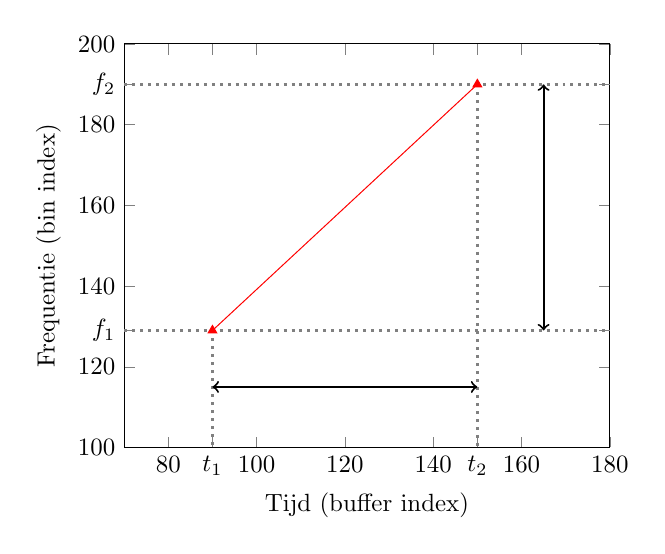
\begin{tikzpicture}[scale=0.9]
\begin{axis}[
	xlabel={Tijd (buffer index)},
	ylabel={Frequentie (bin index)},
	xmin=70,xmax=180,
	ymin=100,ymax=200,
	legend style={
  		cells={anchor=west},
  		legend pos=outer north east,
	},
	extra y ticks={129,190}, 
	extra y tick labels={$f_1$,$f_2$},
	extra x ticks={90,150}, 
	extra x tick labels={$t_1$,$t_2$},
]

  % plot the data from the file data.dat
  % smooth the curve and mark the data point with a dot
  \addplot[color=red,mark=triangle*] coordinates {
  	(90,129)
  	(150,190)
  };
  
  %f1
   \addplot[style= dotted,color=gray,very thick] coordinates{ (70,129)
   (180,129)};
   %f2
   \addplot[style= dotted,color=gray,very thick] coordinates{ (70,190)
   (180,190)};
   
    \node at (99,60) [] {\small$\Delta f$};
    \addplot[color=black,<->,thick] coordinates{ (165,129) (165,190)};
    
   \node at (50,18) [] {\small$\Delta t$};
   \addplot[style=dotted,color=gray,very thick] coordinates{ (90,129)
   (90,100)}; 
   \addplot[style=dotted,color=gray,very thick] coordinates{
   (150,190) (150,100)};
   \addplot[color=black,<->,thick] coordinates{ (90,115)
   (150,115)};
  
  \end{axis}
\end{tikzpicture}
	\end{center}
	\label{schematische-fingerprint}
\end{figure}

Bij het zoeken naar matches kan er gesteund worden op enkele typische eigenschappen van fingerprints: 

Twee overeenkomende fingerprints uit twee geluidsfragmenten zullen dezelfde frequenties  ($f1$ en $f2$) hebben. Bijgevolg is ook het verschil in frequentie ($\Delta f$) gelijk. 

De tijd van de spectrale pieken ($t1$ en $t2$) komen meestal niet overeen. Bij Shazam is het bijvoorbeeld geen vereiste om een opname te maken vanaf het begin van een liedje. Het moment van de opname mag volledig willekeurig worden gekozen. Bij het synchroniseren van streams wordt gezocht naar het verschil tussen de begintijden ($t1$ van elke fingerprint) van de overeenkomstige fingerprints van de audiofragmenten. Dit tijdverschil is wel gelijk bij elk paar overeenkomende fingerprints.

Hoewel de tijd ($t1$ en $t2$) van twee fingerprints meestal verschilt is dit niet het geval voor het verschil ervan ($\Delta t$). Bij twee overeenkomende fingerprints van twee audiofragmenten is het verschil in frequentie inherent gelijk.

Uit voorgaande eigenschappen kan geconcludeerd worden dat fingerprints uit twee audiofragmenten matchen wanneer $ f1 $, $ \Delta f $ en $ \Delta t $ gelijk zijn. Om deze parameters snel met elkaar kunnen te vergelijken wordt er een berekening uitgevoerd die deze parameters omzet in één enkel getal. Dit getal wordt de hash van de fingerprint genoemd. Samen met deze hash wordt ook $ t1 $ en een identificatie van het geluidsfragment bijgehouden.

Artikel \cite{six2014panako} geeft meer informatie over de omzetting van deze drie getallen tot een hash.

Een fingerprint kan bijgevolg gezien worden als verzameling gegevens met de volgende structuur: $ ( id; t1; hash(f1; \Delta f; \Delta t) ) $. Het zoeken naar fingerprints met overeenkomstige hashwaarden is mogelijk in $O(1)$ door gebruik te maken van een hashtabel. De precieze werking hiervan valt buiten de scope van deze scriptie.

Om te bepalen of twee audiofragmenten wel degelijk overeenkomen wordt er gezocht naar alle fingerprints met een overeenkomende hashwaarde. Van elk paar overeenkomende fingerprints wordt het verschil tussen $ t1 $ berekend. Dit verschil wordt de offset genoemd. Het vinden van een groot aantal matches met dezelfde offset wijst op een sterke gelijkenis tussen de audiofragmenten. De precieze waarde van ``een groot aantal'' wordt bepaald door een parameter van het algoritme.

\subsubsection{Bepalen van de latency}

Accoustic fingerprinting kan gebruikt worden om streams te synchroniseren door de ze eerst te bufferen. Wanneer een buffer volledig is opgevuld kan deze net zoals een kort audiofragment worden verwerkt door het algoritme. De latency tussen streams wordt bepaald door de offset die in vorig paragraaf werd beschreven: het verschil tussen de $ t1 $ waarden stelt namelijk de verschuiving tussen de geluidsfragmenten voor.

Figuur \ref{schematische-synchronisatie} toont schematisch alle stappen die moeten worden doorlopen om met behulp van accoustic fingerprinting audiostreams te synchroniseren.

\vspace{0.3cm}
\begin{figure}[h]
	\captionsetup{width=0.7\textwidth}
	\caption[Schema synchronisatie met fingerprinting]{Schematische voorstelling van synchronisatie met behulp van een accoustic fingerprinting systeem.}
	\advance\parskip0.5cm
	\begin{tikzpicture}[overlay]
\node at (-1,0) [minimum width=2cm] (A) {};

\node (rect) at (3,0) [draw,thin,minimum width=3cm,minimum height=1cm,align=center,font=\footnotesize] (B) {Feature \\[-0.7em] extractie};

\node (rect) at (8,0) [draw,thin,minimum width=3cm,minimum height=1cm,align=center,font=\footnotesize] (C) {Fingerprint \\[-0.7em] constructie};

\node (rect) at (13,-2) [draw,thin,minimum width=3cm,minimum height=1cm,align=center,font=\footnotesize] (G) {Andere \\[-0.7em] fingerprints};

\node (rect) at (13,0) [draw,thin,minimum width=3cm,minimum height=1cm,align=center,font=\footnotesize] (D) {Matchen en \\[-0.7em] bepalen latency};

\node at (17,0) [minimum width=2cm] (E) {};

\node at (0,-10) [minimum height=5cm] (F) {};

\draw [->] (A) -- (B) node [pos=0.4,above,align=center,font=\footnotesize] {Buffer};
\draw [->] (B) -- (C) node [pos=0.5,above,align=center,font=\footnotesize] {Features};
\draw [->] (C) -- (D) node [pos=0.5,above,align=center,font=\footnotesize] {Fingerprint};
\draw [->] (D) -- (E) node [pos=0.6,above,align=center,font=\footnotesize] {Latency};
\draw [->] (G) -- (D);

\end{tikzpicture}
	\advance\parskip1cm
	\label{schematische-synchronisatie}
\end{figure}
\vspace{2.5cm}

Een uitgebreidere beschrijving is te vinden in artikel \cite{Wang2003a}. De methode die in het artikel en deze scriptie besproken werd is beperkt tot het vergelijken van audiofragmenten die in tijd noch toonhoogte gewijzigd zijn. Aan het IPEM is een aangepaste methode ontwikkeld die dit wel toelaat \cite{six2014panako}.

\subsubsection{Nauwkeurigheid}

Zowel de snelheid waarmee wijzigingen van de latency bepaald kunnen worden als de nauwkeurigheid van de latency zelf hangt af van heel wat verschillende parameters van het algoritme.

De detectiesnelheid is vooral afhankelijk van de buffergrootte waarop het algoritme wordt uitgevoerd. Met deze instelling moet echter omzichtig worden omgegaan: een te kleine buffergrootte kan er toe leiden dat het algoritme niet meer in staat is om voldoende matches te vinden. Het kan helpen om andere parameters te wijzigen waardoor het vinden van een groot aantal matches gegarandeerd blijft. Deze parameters worden in sectie \ref{accoustic-fingerprinting-params} in detail besproken.

De nauwkeurigheid van de latency van het algoritme hangt af van de parameters van het FFT algoritme. Een nauwkeurigheid van 16 ms of 32 ms is standaard. De precieze werking van het FFT algoritme valt buiten de scope van deze scriptie.

\subsection{Kruiscovariantie}
\label{kruiscovariantie}

Deze methode bepaalt de gelijkenis tussen twee audiofragmenten en resulteert in één getal. Dit getal is een soort van score die aangeeft in welke mate twee signalen overeenkomen. De latency tussen twee audiofragmenten kan bepaald worden door deze berekening uit te voeren voor \textbf{elke mogelijke verschuiving}. De verschuiving waarbij het resulterend getal het hoogst is bepaalt de latency.

\subsubsection{Werking}

Stel twee audioblokken $ a $ en $ b $ bestaande uit een gelijk aantal samples ($n$). Deze audioblokken worden telkens cyclisch één sample verschoven tot wanneer de kruiscovariantie waarde ($ k $) voor elke mogelijke verschuiving berekend werd. De variabele $ i $ stelt de huidige verschuiving voor en gaat van 0 tot $ n $. De kruiscovariantie wordt berekend met formule:

\begin{equation}
	k = \sum_{j=0}^{n} a_{j} \cdot b_{(i+j) \bmod n}
\end{equation}

De waarde van $ i $ waarbij de kruiscovariantie het hoogst is stelt de latency voor tussen beide audioblokken in aantal samples. De latency in seconden kan bepaald worden door dit resultaat te delen door de samplefrequentie.

De methode kan de latency \textbf{tot op één sample nauwkeurig} bepalen. De maximaal bereikbare nauwkeurigheid hangt dus af van de samplefrequentie van de audioblokken. Bij een samplefrequentie van $8000 Hz$ is dit $ 1/8000 Hz = 0.125 ms $. Dit is ruim voldoende voor het huidige probleem.

Een nadeel aan deze methode is de performantie. Het berekenen van de beste kruiscovariantie van twee audioblokken bestaande uit $ n $ samples kan gebeuren in  $O(n^{2})$. Het is dus belangrijk om bij deze berekening de grootte van de audioblokken te beperken.

In artikel \cite{six2015multimodal} wordt deze techniek meer in detail besproken.

\subsubsection{Toepassing in realtime}

Het bufferen van de audiostreams maakt ook dit algoritme in realtime toepasbaar. In tegenstelling tot accoustic fingerprinting is het niet de bedoeling dat de berekeningen op de volledige buffer wordt uitgevoerd. Door de kwadratische tijdscomplexiteit zou het algoritme onnoemelijk veel rekenkracht vragen.\footnote{Voor het berekenen van de kruiscovariantie tussen twee buffers met $10s$ audio en een samplefrequentie van $8000hz$ zijn er asymptotisch $ 6.4 \cdot 10^9 $ berekeningen vereist.} Er moet dus een manier gevonden worden waarmee het mogelijk is om het aantal samples waarop het algoritme wordt uitgevoerd beperkt wordt.

\subsection{Toepasbaarheid}
\label{toepasbaarheid}

Het accoustic fingerprinting algoritme is zeer snel en robuust en kan gebruikt worden om gebufferde audiostreams te synchroniseren tot enkele tientallen milliseconden nauwkeurig (afhankelijk van de parameters van het FFT algoritme).

Het kruiscovariantie algoritme kan eveneens gebruikt worden om (gebufferde) audiostreams te synchroniseren. De grootste troef van dit algoritme is haar nauwkeurigheid: in de beste omstandigheden kan het algoritme resultaten bekomen tot op één sample nauwkeurig. Het bereiken van een dergelijke nauwkeurigheid is onmogelijk met eender welk ander besproken algoritme. De keerzijde is de performantie van het algoritme. Bij het synchroniseren van grote audioblokken kan dit problematisch zijn.

De kenmerken van deze algoritmen zijn complementair. De gemakkelijkste manier om een robuust, snel én nauwkeurig systeem op te bouwen is door het beste van de twee werelden te combineren. Het accoustic fingerprinting algoritme kan zorgen voor de synchronisatie tot op enkele tientallen milliseconden nauwkeurig. Dit resultaat laat toe dat we het kruiscovariantie algoritme kunnen uitvoeren op zeer korte stukjes audio (een honderdtal milliseconden volstaat).

\section{Bufferen van streams}
\label{streambuffers}

Aangezien de algoritmes een bepaalde hoeveelheid audio nodig hebben vooraleer ze kunnen worden uitgevoerd is het noodzakelijk om de streams eerst te bufferen. Dit proces moet herhaald worden aangezien er mogelijk samples gedropt worden of drift kan ontstaan. In dit deel zal worden uitgelegd hoe het bufferen precies in zijn werk gaat. Om verwarring met andere soorten buffers te vermijden zal dit type buffer verder in deze scriptie een \textit{streambuffer} genoemd worden.

\subsubsection{Buffergrootte}

De grootte van de buffer heeft invloed op de kwaliteit van de resultaten. Het spreekt voor zich dat het algoritme beter kan presteren wanneer er 10 seconden in plaats van 1 seconde audio geanalyseerd wordt. Een nadeel is echter dat het langer duurt vooraleer een wijzing van de latency gedetecteerd kan worden. 

\subsubsection{Naïeve implementatie}

De naïeve implementatie kan een wijziging van de latency in het beste geval na $ \frac{1}{2} t $ seconden detecteren. Wanneer er samples gedropt worden net voor het moment dat de buffer voor de helft gevuld is, dan kan het algoritme de nieuwe latency wel onmiddellijk detecteren.

\subsubsection{Sliding window}

Een meer doordachte manier van bufferen maakt gebruik van een \textit{sliding window}. In onderstaande beschrijving wordt gebruik gemaakt van een buffer met $ t $ seconden capaciteit en een stapgrootte van $ s $ seconden, hierbij geldt dat $ s \leq t $. 

Het verschil met de naïeve methode is dat de buffer niet pas na $ t $ seconden wordt opgeschoven. Door de buffer al na $ s $ seconden op te schuiven zal een wijziging van de latency sneller gedetecteerd kunnen worden; dit terwijl het algoritme toch nog steeds $ t $ seconden audio kan analyseren. In figuur \ref{slidingwindow} wordt grafisch weergegeven hoe de buffer precies verschoven wordt met $ t = 10 $ en $ s = 5 $.

\begin{figure}[h!]
	\captionsetup{width=0.7\textwidth}
	\caption[Schematische weergave van de buffer]{Schematische weergave van een \textit{sliding window} buffer over een audiostream.}
	\begin{center}
		\advance\parskip0.3cm
		\begin{tikzpicture}[scale=0.9]
\begin{axis}[
xlabel={Tijd (seconden)},
xmin=170,xmax=200,
ymin=0,ymax=1,
legend style={
	cells={anchor=west},
	legend pos=outer north east,
},
yticklabels={,,},
xticklabel style={grid=major},
extra x ticks={176,177,186,187},
extra x tick labels={,,,},
extra tick style={grid=major, grid style={dotted}},
hide y axis
]
\addplot[thick,black] graphics[xmin=140,ymin=0,xmax=200,ymax=1] {wave.png};

after end axis/.code={
	\draw[black,<->] (axis cs:175,0.1) -- (axis cs:185,0.1)	node [pos=0.5,above,font=\scriptsize] {buffer $i-1$};
	
	\draw[black,<->] (axis cs:176,0.2) -- (axis cs:186,0.2)	node [pos=0.5,above,font=\scriptsize] {buffer $i$};
	
	\draw[black,<->] (axis cs:177,0.3) -- (axis cs:187,0.3)	node [pos=0.5,above,font=\scriptsize] {buffer $i+1$};
}]

%\node at (50,18) [] {\small$\Delta t$};
%\addplot[style=dotted,color=gray,very thick] coordinates{ (90,129)
%	(90,100)}; 
%\addplot[style=dotted,color=gray,very thick] coordinates{
%	(150,190) (150,100)};
%\addplot[color=black,<->,thick] coordinates{ (90,115)
%	(150,115)};

\end{axis}

\end{tikzpicture}
	\end{center}
	\label{slidingwindow}
\end{figure}

Door de buffer al na $ s $ seconden op te schuiven wordt het slechtste geval sterk verbeterd. In het slechtste geval wordt een wijziging van de latency gedetecteerd na $ \frac{t}{2} + s $ seconden. Het beste geval blijft wel nog steeds $ \frac{t}{2} $ seconden.

Het verkleinen van de stapgrootte zorgt ervoor dat het algoritme per hoeveelheid audio frequenter moet worden uitgevoerd. Een te kleine stapgrootte heeft bijgevolg een negatieve invloed op de performantie.

\subsubsection{Voorbeeld}

Een praktisch voorbeeld zal bovenstaande beschrijving wat verduidelijken. In het voorbeeld worden twee audiostreams van 40 seconden geanalyseerd. Door het droppen van samples neemt de latency tussen de streams stapsgewijs toe. Figuur \ref{latency} toont in het zwart hoe de latency gedurende de verwerking evolueert. De opeenvolgende buffers van de twee besproken methode's worden in het rood aangeduid. 

\begin{figure}[h!]
	\captionsetup{width=0.7\textwidth}
	\caption[Voorbeeld buffering methodes]{Grafisch weergave van de methode's waarop gebufferd kan worden. De zwarte lijn stelt de huidige latency voor. In het rood worden de opeenvolgende buffers weergegeven.}
	\begin{center}
		\advance\parskip0.3cm
		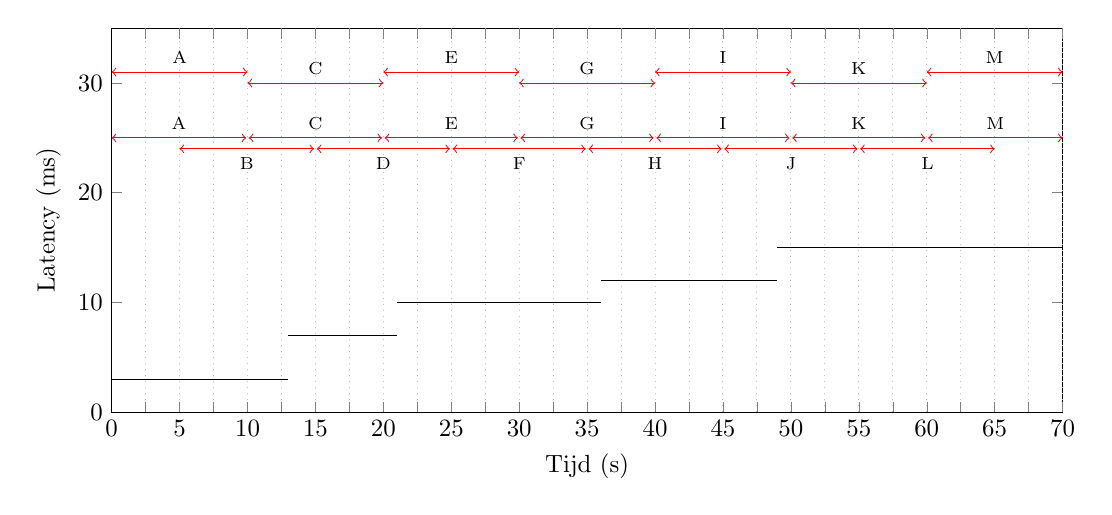
\begin{tikzpicture}[scale=0.9]
\begin{axis}[
xlabel={Tijd (s)},
ylabel={Latency (ms)},
xmin=0,xmax=70,
ymin=0,ymax=35,
legend style={
	cells={anchor=west},
	legend pos=outer north east,
},
extra x ticks ={2.5,5,7.5,...,70},
extra x tick labels={,,,},
extra x tick style={grid=major, grid style={dotted}},
width = 15cm,
height = 7cm
]



after end axis/.code={
	\draw (axis cs:0,3) -- (axis cs:13,3);
	\draw (axis cs:13,7) -- (axis cs:21,7);
	\draw (axis cs:21,10) -- (axis cs:36,10);
	\draw (axis cs:36,12) -- (axis cs:49,12);
	\draw (axis cs:49,15) -- (axis cs:70,15);
	
	\draw[red,<->] (axis cs:0,31) -- (axis cs:10,31)	node [pos=0.5,above,font=\scriptsize,color=black] {A};
	\draw[red,<->] (axis cs:10,30) -- (axis cs:20,30)	node [pos=0.5,above,font=\scriptsize,color=black] {C};
	\draw[red,<->] (axis cs:20,31) -- (axis cs:30,31)	node [pos=0.5,above,font=\scriptsize,color=black] {E};
	\draw[red,<->] (axis cs:30,30) -- (axis cs:40,30)	node [pos=0.5,above,font=\scriptsize,color=black] {G};
	\draw[red,<->] (axis cs:40,31) -- (axis cs:50,31)	node [pos=0.5,above,font=\scriptsize,color=black] {I};
	\draw[red,<->] (axis cs:50,30) -- (axis cs:60,30)	node [pos=0.5,above,font=\scriptsize,color=black] {K};
	\draw[red,<->] (axis cs:60,31) -- (axis cs:70,31)	node [pos=0.5,above,font=\scriptsize,color=black] {M};
	
	\draw[red,<->] (axis cs:0,25) -- (axis cs:9.9,25)	node [pos=0.5,above,font=\scriptsize,color=black] {A};
	\draw[red,<->] (axis cs:5,24) -- (axis cs:14.9,24)	node [pos=0.5,below,font=\scriptsize,color=black] {B};
	\draw[red,<->] (axis cs:10.1,25) -- (axis cs:19.9,25)	node [pos=0.5,above,font=\scriptsize,color=black] {C};
	\draw[red,<->] (axis cs:15.1,24) -- (axis cs:24.9,24)	node [pos=0.5,below,font=\scriptsize,color=black] {D};
	\draw[red,<->] (axis cs:20.1,25) -- (axis cs:29.9,25)	node [pos=0.5,above,font=\scriptsize,color=black] {E};
	\draw[red,<->] (axis cs:25.1,24) -- (axis cs:34.9,24)	node [pos=0.5,below,font=\scriptsize,color=black] {F};
	\draw[red,<->] (axis cs:30.1,25) -- (axis cs:39.9,25)	node [pos=0.5,above,font=\scriptsize,color=black] {G};
	\draw[red,<->] (axis cs:35.1,24) -- (axis cs:44.9,24)	node [pos=0.5,below,font=\scriptsize,color=black] {H};
	\draw[red,<->] (axis cs:40.1,25) -- (axis cs:49.9,25)	node [pos=0.5,above,font=\scriptsize,color=black] {I};
	\draw[red,<->] (axis cs:45.1,24) -- (axis cs:54.9,24)	node [pos=0.5,below,font=\scriptsize,color=black] {J};
	\draw[red,<->] (axis cs:50.1,25) -- (axis cs:59.9,25)	node [pos=0.5,above,font=\scriptsize,color=black] {K};
	\draw[red,<->] (axis cs:55.1,24) -- (axis cs:65,24)	node [pos=0.5,below,font=\scriptsize,color=black] {L};
	\draw[red,<->] (axis cs:60.1,25) -- (axis cs:70,25)	node [pos=0.5,above,font=\scriptsize,color=black] {M};
	
%	\draw[black,<->] (axis cs:10,0.2) -- (axis cs:20,0.2)	node [pos=0.5,above,font=\scriptsize] {buffer $i$};
	
%	\draw[black,<->] (axis cs:20,0.3) -- (axis cs:30,0.3)	node [pos=0.5,above,font=\scriptsize] {buffer $i+1$};
}]

\end{axis}

\end{tikzpicture}
	\end{center}
	\label{latency}
\end{figure}

De initiële latency van 3 milliseconden wordt zowel met de naïeve methode als met het sliding window gedetecteerd na de analyse van de allereerste buffer (A of R) 10 seconden na aanvang van de analyse. De eerste verhoging tot 7 milliseconden vindt te laat plaats om gedetecteerd te kunnen worden door de eerste buffer van beide methodes. Bij deze verhoging van de latency wordt het verschil tussen beide methodes zichtbaar: bij  de sliding window methode vindt de detectie 6 seconden na de wijziging plaats. Bij de naïeve methode moet er echter gewacht worden tot wanneer buffer B is volgelopen 12 seconden na de wijziging. De tweede verhoging naar 10 milliseconden wordt zowel door de naïeve methode als door de sliding window methode gedetecteerd 8 seconden na de wijziging (buffer C of W). 

\subsubsection{Conclusie}

De detectiesnelheid van een latencywijziging hangt af van twee parameters: de bufferlengte ($t$) en de staplengte ($s$). De snelheid waarmee een wijziging gedetecteerd kan worden ($ T $) kan als volgt worden samengevat:

\begin{equation}
	\frac{t}{2} < T < \frac{t}{2} + s
\end{equation}

Het toepassen van deze formules op het vorige paragraaf levert volgende resultaten: Zowel bij de naïeve als sliding window methode is de ondergrens 5 seconden. De bovengrens bij de naïeve methode bedraagt 15 seconden. Bij de sliding window methode is dit begrenst tot 9 seconden.

\section{Synchroniseren van streams}

In deze toepassing wordt de latency van alle streams bepaald ten opzichte van een referentiestream. Het is niet geweten welke stream voorloopt of achterloopt. Wanneer de referentiestream een bepaalde vertraging heeft ten opzichte van een andere stream dan zal de latency van de andere stream negatief zijn. Bij de daadwerkelijke synchronisatie is het belangrijk dat hiermee rekening gehouden wordt.

\subsubsection{Algoritme}

Elke keer wanneer er een nieuwe verzameling latencies (ten opzichte van de referentiestream) bepaald is moeten de streams worden aangepast. Dit gebeurt door het toevoegen van stilte (samples met waarde 0.0). Het volgende algoritme berekent hoeveel stilte aan welke streams moet worden toegevoegd.

\begin{algorithm}
	\setstretch{1}
	\label{sync-algo}
	\begin{algorithmic}[1] % The number tells where the line numbering should start
		\Function{Correcties}{$L, P$} \Comment{L: lijst van latencies, P: lijst van vorige latencies}
		\State $n\gets$ lengte van $L$ en $P$
		\State $h\gets -\infty$ \Comment{h: de huidige hoogste correctie}
		\State $C_i\gets$ lege lijst \Comment{lijst met de correcties van elke stream}
		\For{$i\gets 1..n$}
			\State $l\gets$ aantal samples in $L_i$
			\State $p\gets$ aantal samples in $P_i$
			\State $c\gets l - p $ \Comment{c: correctie in samples van stream $ i $}
			\If{$c > h$}
				\State $h\gets c$ \Comment{wijzigen van hoogste correctie}
			\EndIf
			\State $C_i\gets c$
		\EndFor
		
		\For{$i\gets 1..n$}
			\State $C_i\gets h - C_i$\Comment{correctie wordt relatief t.o.v. hoogste correctie}
		\EndFor
		\State \textbf{return} $C$
		\EndFunction
	\end{algorithmic}
\end{algorithm}

In het algoritme wordt op basis van de nieuwe en vorige verzameling van latencies per stream de correctie bepaald. Dit is het aantal nul-samples die aan de overeenkomstige stream moet worden toegevoegd. Bij de eerste berekening (regel 8) is het mogelijk dat de correctie negatief is. Aangezien we geen extra audio willen verliezen (samples wegknippen) wordt de correctie omgezet zodat deze relatief is ten opzichte van de hoogste correctie (regel 16). 

Door het berekende aantal nul-samples aan elke stream toe te voegen worden de streams gesynchroniseerd.